\makeatletter\let\ifGm@compatii\relax\makeatother
\documentclass[mathserif,fleqn]{beamer}

\mode<presentation>
{
  %\usetheme{Warsaw}
  \usetheme{Antibes}
  %\usetheme{Boadilla}
  \setbeamercovered{transparent}
}
%\usepackage{beamerthemesplit}
\usepackage{beamerthemeshadow}
%\usepackage[width=2cm,dark,tab]{beamerthemesidebar}

\usepackage{pgf,pgfarrows,pgfnodes,pgfautomata,pgfheaps}
%\usepackage[tbtags]{amsmath}
\usepackage{amsmath,amssymb,amsfonts}
\usepackage{color,xcolor}
\usepackage{graphicx}
\usepackage{multimedia}
\usepackage{manfnt}
\usepackage[english]{babel}
\usepackage{algorithmic}
\usepackage{algorithm}
\usepackage{setspace}
\usepackage[timeinterval=1]{tdclock}
\usepackage{tikz}
\usetikzlibrary{shapes,arrows}
%\beamersetaveragebackground{black!10}
\usefonttheme[stillsansseriflarge]{serif}
\usepackage{times}
\beamertemplatesolidbackgroundcolor{white}
%\beamertemplateshadingbackground{white!90}{structure!1}
%\beamertemplatesolidbackgroundcolor{white!90!blue}
\beamertemplatetransparentcovereddynamic
\beamertemplateballitem
\beamertemplatenumberedballsectiontoc
%\beamertemplatelargetitlepage
\beamertemplateboldpartpage
\setbeamertemplate{itemize item}[triangle]
%\setbeamertemplate{footline}[page number]
\setbeamertemplate{footline}[text line]{%
\llap{Songpeng Zu\hspace{-5mm}}\centerline{\strut Machine Learning on Compound-Protein Interactions}\llap{\insertframenumber\hspace{-5mm}}}
\newtheorem{jiashe}{Assumption~}[section]


%\setbeamertemplate{item}[triangle]
\graphicspath{{./figures/}}
%\AtBeginSection[]{
%  \frame<handout:0>{
%    \frametitle{Content}
%    \tableofcontents[current,currentsubsection]
%  }
%}
%\AtBeginSubsection[]{
%  \frame<handout:0>{
%    \frametitle{Content}
%    \tableofcontents[current,currentsubsection]
%  }
%}
% Table rules
\def\toprule{\noalign{\ifnum0=`}\fi\hrule \@height 0.5pt \hrule \@height 6pt \@width 0pt \futurelet
   \@tempa\@xhline}
\def\midrule{\noalign{\ifnum0=`}\fi \hrule \@height 6.75pt \@width 0pt \hrule \@height 0.5pt
    \hrule \@height 6pt \@width 0pt \xfuturelet \@tempa\@xhline}
\def\botrule{\noalign{\ifnum0=`}\fi \hrule \@height 5.75pt \@width 0pt \hrule \@height 0.5pt \futurelet
   \@tempa\@xhline}

% Define block styles
\tikzstyle{decision} = [diamond, draw, fill=blue!20,
    text width=4.5em, text badly centered, node distance=2.5cm, inner sep=0pt]
\tikzstyle{block} = [rectangle, draw, fill=blue!20,
    text width=5em, text centered, rounded corners, minimum height=4em]
\tikzstyle{line} = [draw, -latex']
\tikzstyle{cloud} = [draw, ellipse,fill=red!20, node distance=2.5cm,
    minimum height=2em]


\begin{document}

\title{Qualitatively Predicting Compound-Protein Interactions by Multi-Task Learning}
\author[zusp]{Songpeng Zu\\
zusongpeng@gmail.com
%advisor: shao li
}
%\institute[tnlist]{
%  fit 1-108,  tsinghua university\\
%}
%\date[\initclock\mmddyyyy\tddate\ \ \hhmmss\tdtime]{\today}
\date[\initclock\tdtime]{\today}
%\maketitle
\frame[plain]{\titlepage}

\section*{outline}
\frame{
    \setbeamercolor{uppercol}{fg=white,bg=teal}
    %\setbeamercolor{lowercol}{fg=black,bg=lime}
    \begin{beamerboxesrounded}[upper=uppercol,shadow=true]{outline}
    \begin{spacing}{1.2}
      \begin{itemize}
      \item
        Background:
        \begin{itemize}
        \item Quantitative Structure-Activity Relationship (QSAR)
        \item Multi-task Learning
        \end{itemize}
      \item
        Method: hierarchical Bayesian model called MultiQSAR
      \item
        Result: reduce MSE on PeptideGPCR
      \item
        Discussion: other multi-task models.
    \end{itemize}
    \end{spacing}
    \end{beamerboxesrounded}
}
\part{Quantitatively predicting compound-protein interactions by multi-task learning}
\frame{\partpage}
\section{Background}
\subsection{Methods for CPIs}
\frame{
\frametitle{background}
    Methods for predicting compound-protein interactions (CPIs):
        \begin{itemize}
          \item
          \textcolor{red}{structure-based molecular dynamics}
          \begin{itemize}
            \item depend on proteins' 3D structures.
         %   \item cost too much time
          \end{itemize}
          \item
          \textcolor{red}{ligand-based method}
          \begin{itemize}
            \item  can be independent of proteins' 3d structures.
            \item  large-scale known CPIs data
            \item  mainly dependent on machine learning approaches.
          \end{itemize}
       \end{itemize}
}
\subsection{Machine learning on CPIs}
\frame{
\frametitle{Machine learning on CPIs}
\begin{columns}
\begin{column}{0.65\textwidth}
\begin{itemize}
    \item Compounds represented by topological fingerprints. The similar as proteins.
    \item CPIs recorded as binary variable or continuous variables.
    \item Classification or regression models then are used.
  \end{itemize}
\end{column}
\begin{column}{0.5\textwidth}
  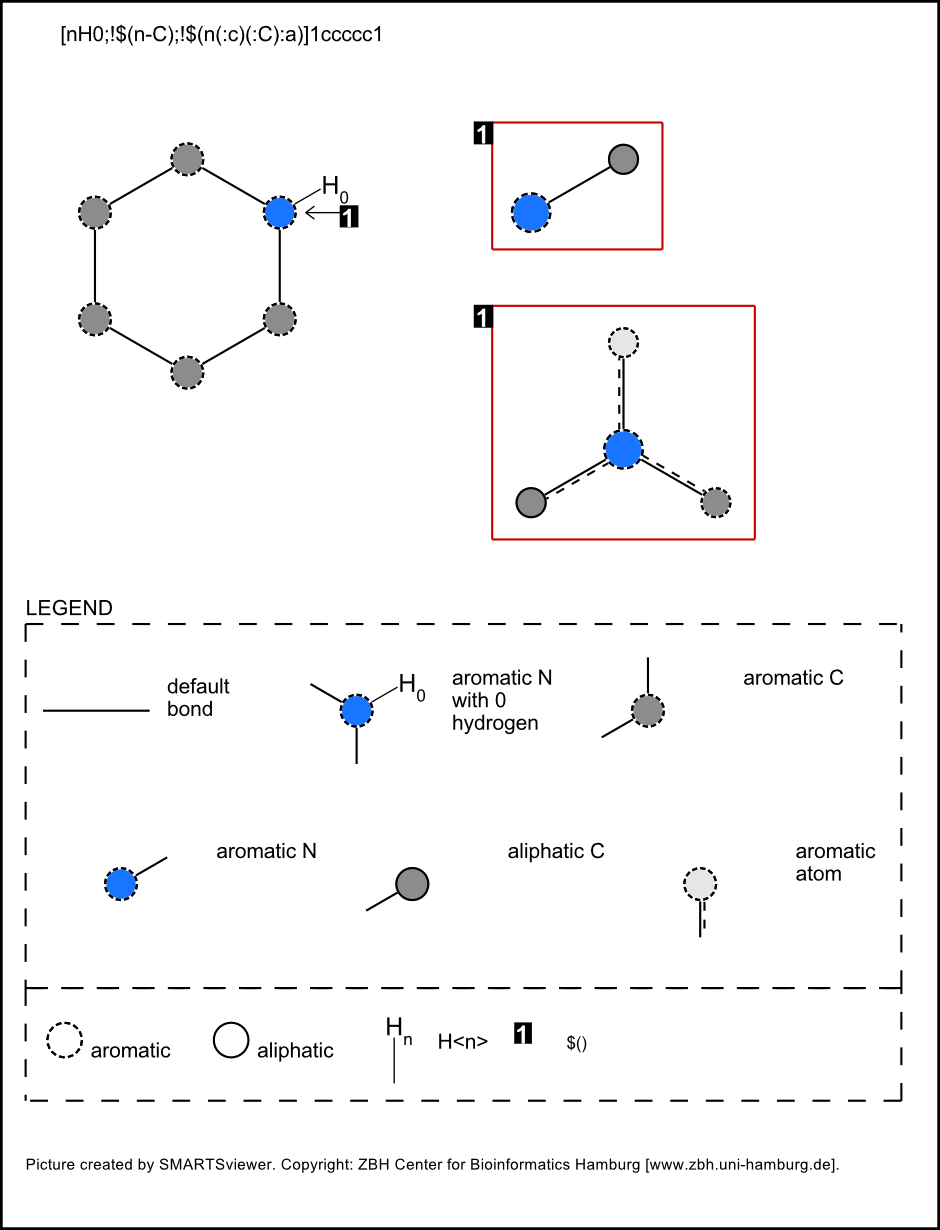
\includegraphics[width=\columnwidth]{exam5}
\end{column}
\end{columns}
}

\frame{
\frametitle{Modeling on a single protein}
Keiser M.J. \textit{et~al}., \textit{Nature} 2009, developed the SEA method to predict drugs' new molecular targets.
\begin{itemize}
\item
Each target represented by its set of known ligands.
\item
Drugs computationally screen against a panel of proteins by comparing the similarity of ligands against these proteins.
\item
The similarities expressed as E-values, adapting the BLAST algorithm.
\end{itemize}}
\frame{
\frametitle{Modeling on a single protein}
Besnard J. \textit{et~al}., \textit{Nature} 2012, used naive Bayesian model to predict compounds' polypharmacology profiling.
\begin{itemize}
  \item
  215,000 activity data including 133,061 compounds and 784 proteins were used.
  \item
  Every compounds represented by the binary vectors of ECFP6 representations.
  \item
  For every protein, a Laplacian-modified naive models was built for classification.
\end{itemize}
}
\frame{

\frametitle{Modeling on a protein family}
\begin{columns}
\begin{column}{0.9\textwidth}
Yabuuchi H. \textit{et~al}., \textit{Molecular Systems Biology} 2011 developed the CGBVS framework.
\begin{itemize}
    \item 5207 CPIs data (including 317 GPCRs and 866 ligands)
    \item Compounds' structure and proteins' sequences converted into 929- and 400-dimensional vectors
    \item SVM then used.
  \end{itemize}
\end{column}
%\begin{column}{0.45\textwidth}
%  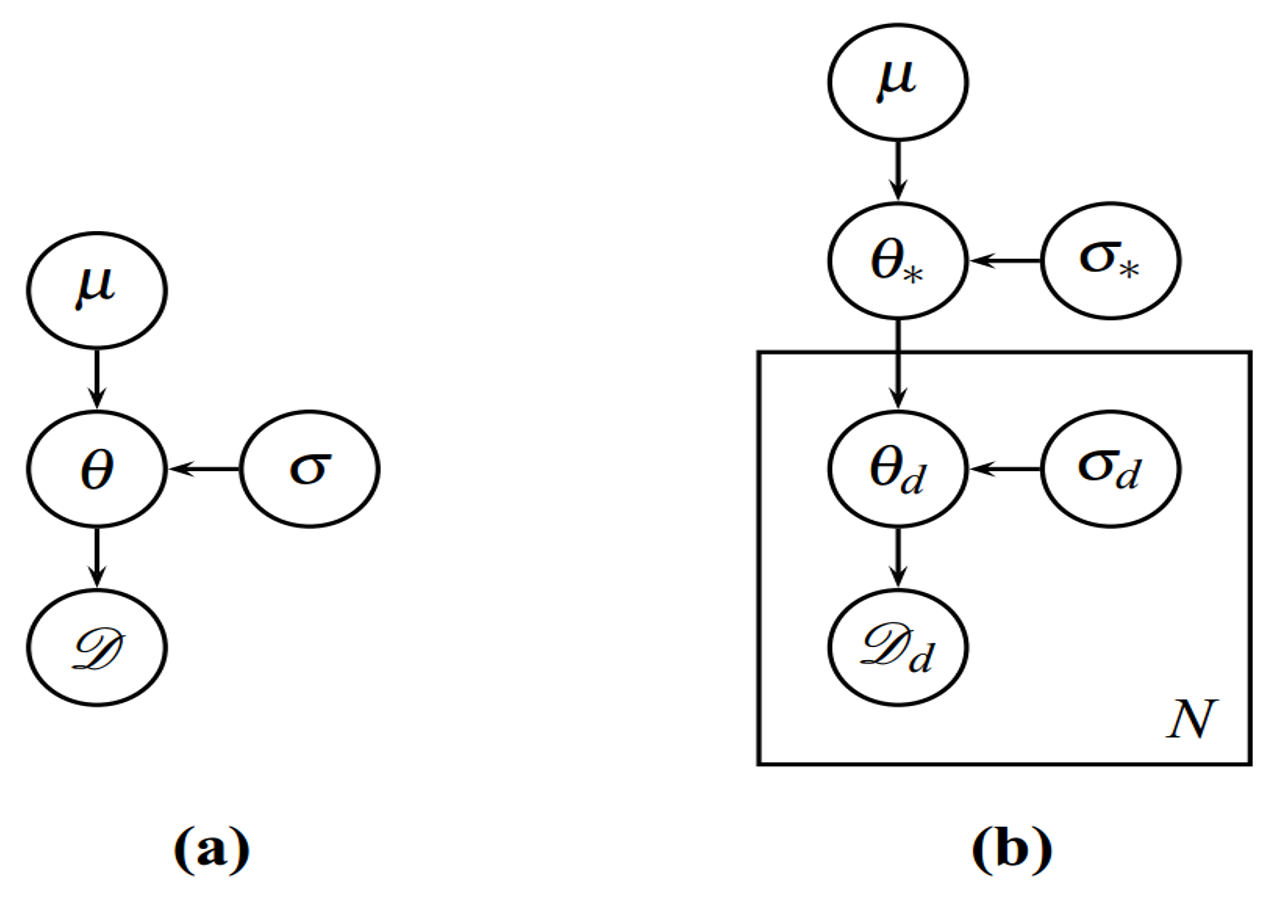
\includegraphics[width=\columnwidth]{hbda} %cgbv
%\end{column}
\end{columns}
}
\frame{
\frametitle{Machine Learning on CPIs}
Current machine learning on predicting CPIs
\begin{itemize}
  \item Modeling on a single protein\\
  \textcolor{blue}{More specificity} \textcolor{red}{Lots of data needed}
  \item Modeling on a protein family\\
  \textcolor{blue}{Data sharing} \textcolor{red}{Less specificity}
\end{itemize}
}
\subsection{Transfer Learning}

\frame{
\frametitle{Multi-Task Learning}
\textcolor{blue}{Can we combine the two approaches ?}
\begin{itemize}
  \item
  Learning different but similar tasks at the same time. (Finkel J.R. and Mannning C.D., 2009)
  \item
  Quantitative prediction.
\end{itemize}
\begin{figure}
\centering
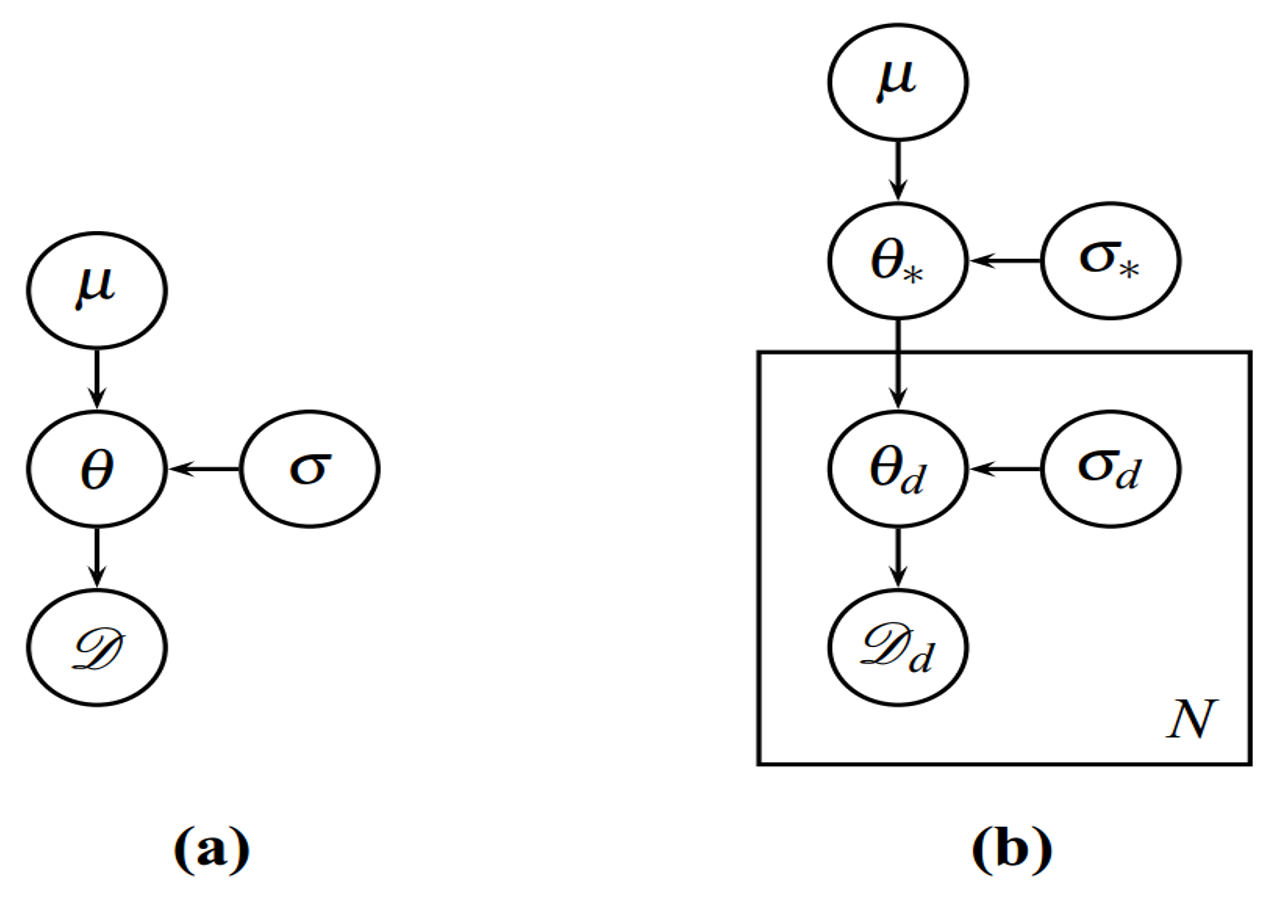
\includegraphics[width=0.55\columnwidth]{hbda}
\end{figure}
}
\section{Method}
\subsection{Mathematical formulation}
\frame{
\frametitle{Hierarchical Bayesian Model}
Suppose $ \mathbf{\mathcal{D}}_{j} = \left\{\textbf{X}_{j},\textbf{y}_{j}\right\},j=1,...,m$, and $\textbf{X}_{j}\in\mathbb{R}^{d\times n_{j}}$. Then we have
\begin{equation}
  \mathbf{y}_{j} \sim \mathcal{N}\left(\mathbf{X}_{j}^{T}\mathbf{\omega}_{j},\sigma_{y}^{2}\mathbf{I}\right)
\end{equation}
Since different groups data may share similar features, we assume $\mathbf{\omega}_{j}$ have the same mean on the prior distribution.
\begin{equation}
  \mathbf{\omega}_{j} \sim \mathcal{N} \left(\mathbf{\omega}_{\ast},\sigma_{j}^{2}\mathbf{I}\right)
\end{equation}
In which,
\begin{equation}
  \mathbf{\omega}_{\ast} \sim \mathcal{N} \left(\mathbf{\mu},\mathbf{\sigma}_{\ast}^2\mathbf{I}\right)
\end{equation}
}
\subsection{Loglikehood Function}
\frame{
Suppose, for simplicity, that $\mathbf{\mu}=\textbf{0}$, $p(\sigma_{y}^2)\propto 1$, and that $\sigma_{j}^2$ and $\sigma_{\ast}$ are fixed. Let
$\Theta = \left\{\mathbf{\omega}_j, j=1,...,m,\mathbf{\omega}_\ast,\sigma_{y}^2\right\}$. We have
\begin{equation}
\small
\begin{aligned}
  &\mathcal{L}_{hier}(\mathcal{D};\Theta) =
  \mathcal{L}_{orig}(\mathcal{D}| \Theta)+ \textit{logp}(\Theta)\\
  &=\sum_{j}\left(\textit{logp}(\mathcal{D}_{j}|\mathbf{\omega}_{j})-\frac{\parallel\mathbf{\omega}_{j}-\mathbf{\omega}_{\ast}\parallel^{2}}{2\sigma_{j}^2}\right)
  -\frac{\parallel\mathbf{\omega}_{\ast}\parallel^{2}}{2\sigma_{\ast}^2}\\
  &- \overbrace{\sum_{j}\frac{d}{2}\textit{log}(2\pi\sigma_{j}^2)-\frac{d}{2}\textit{log}(2\pi\sigma_{\ast}^2)}^{\textit{Const}}\\
  &=\sum_{j}\left(-\frac{\parallel\mathbf{y}_{j}-\mathbf{X}^{T}_{j}\mathbf{\omega}_{j}\parallel^{2}}{2\sigma_{y}^2}-\frac{\parallel\mathbf{\omega}_{j}-\mathbf{\omega}_{\ast}\parallel^{2}}{2\sigma_{j}^2}\right)-
  \frac{\parallel\mathbf{\omega}_{\ast}\parallel^{2}}{2\sigma_{\ast}^2}-\sum_{j}\frac{n_{j}}{2}\textit{log}(2\pi\sigma_{y}^2)\\
  &- \overbrace{\sum_{j}\frac{d}{2}\textit{log}(2\pi\sigma_{j}^2)-\frac{d}{2}\textit{log}(2\pi\sigma_{\ast}^2)}^{\textit{Const}}
\end{aligned}
\end{equation}
}
\subsection{Optimization: L-BFGS-B}
\frame{
L-BFGS-B optimization method is then used following the gradient below.
\begin{equation}
\small
\begin{aligned}
  \frac{\partial\mathcal{L}_{hier}(\mathcal{D};\Theta)}{\partial\mathbf{\omega}_j}
  &= -\frac{1}{2\sigma_{y}^2}\frac{\parallel\mathbf{y}_j-\mathbf{X}_{j}^{T}\mathbf{\omega}_j\parallel^2}{\partial\mathbf{\omega}_j}
  -\frac{1}{2\sigma_{j}^2}\frac{\parallel\mathbf{\omega}_j-\mathbf{\omega}_{\ast}\parallel^{2}}{\partial\mathbf{\omega}_j}\\
  &=\frac{\mathbf{X}_j\mathbf{y}_j}{\sigma_{y}^2}+\frac{\mathbf{\omega}_{\ast}}{\sigma^2_j}-
  \left(\frac{\mathbf{X}_j\mathbf{X}_j^{T}}{\sigma_{y}^2}+\frac{1}{\sigma_{j}^2}\mathbf{I}\right)\mathbf{\omega}_{j}
\end{aligned}
\end{equation}
\begin{equation}
\small
  \frac{\partial\mathcal{L}_{hier}(\mathcal{D};\Theta)}{\partial\mathbf{\omega}_{\ast}}
  =-\sum_j\frac{\mathbf{\omega}_{\ast}-\mathbf{\omega}_j}{\sigma_{j}^2}-\frac{\mathbf{\omega}_{\ast}}{\sigma_{\ast}^2}
\end{equation}
\begin{equation}
\small
  \frac{\partial\mathcal{L}_{hier}(\mathcal{D};\Theta)}{\partial\sigma_{y}^2}
  =\frac{\sum_j\parallel\mathbf{y}_j-\mathbf{X}_{j}^{T}\mathbf{\omega}_j\parallel^2}{2(\sigma_{y}^2)^2}-\frac{n}{2\sigma_{y}^2}
\end{equation}
where n is the total number of samples in all the groups.
}
\subsection{Data Sets}
\frame{
%\frametitle{Data Sets}
\begin{itemize}
  \item 210,000 CPIs including more than 1,000 proteins from 20 protein families, and  150,000 compounds.
  \item 22 physicochemical properties and 881 chemical substructures as the compounds' features.
\end{itemize}
\begin{figure}
  \centering
  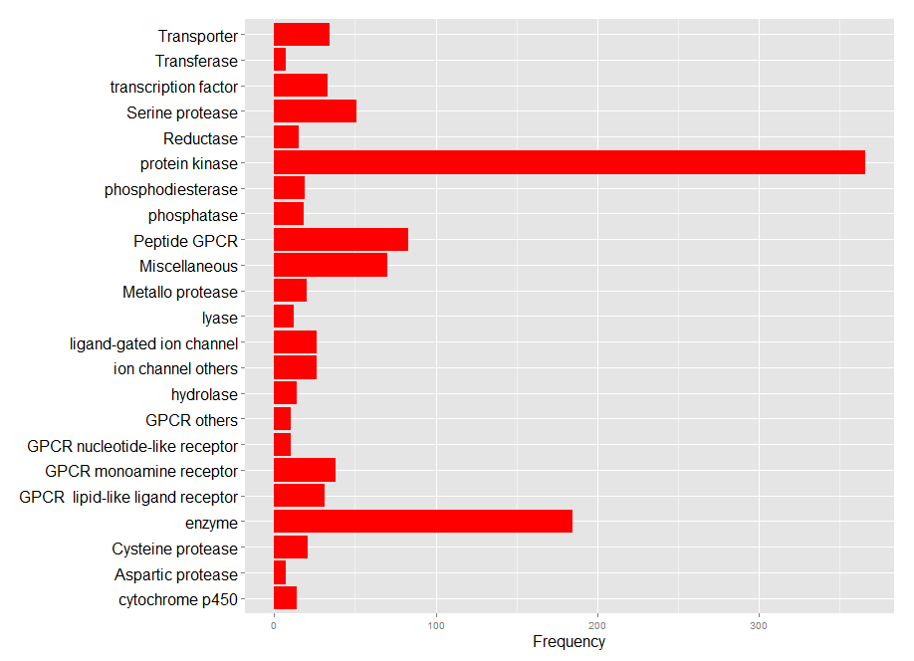
\includegraphics[width=0.75\columnwidth]{pfamily}
\end{figure}
}
\section{Result}
\subsection{Feature Selection}
\frame{
\frametitle{Feature Selection}
The protein family of Peptide GPCR including 85 proteins as examples.
\begin{itemize}
  \item
  Based on the definitions of chemical fingerprints, SUB1-SUB115, SUB264-SUB327 are removed.
  \item
  Chemical fingerprints with too low or high frequencies are removed.
  \item
  Non-parametric dynamic slicing method for marginal feature selection.
  \item
  284 features are finally kept.
\end{itemize}
}
%\subsection{Learning Pattern}
%\frame{
%%\frametitle{Learning Pattern}
%\begin{figure}
%  \centering
%  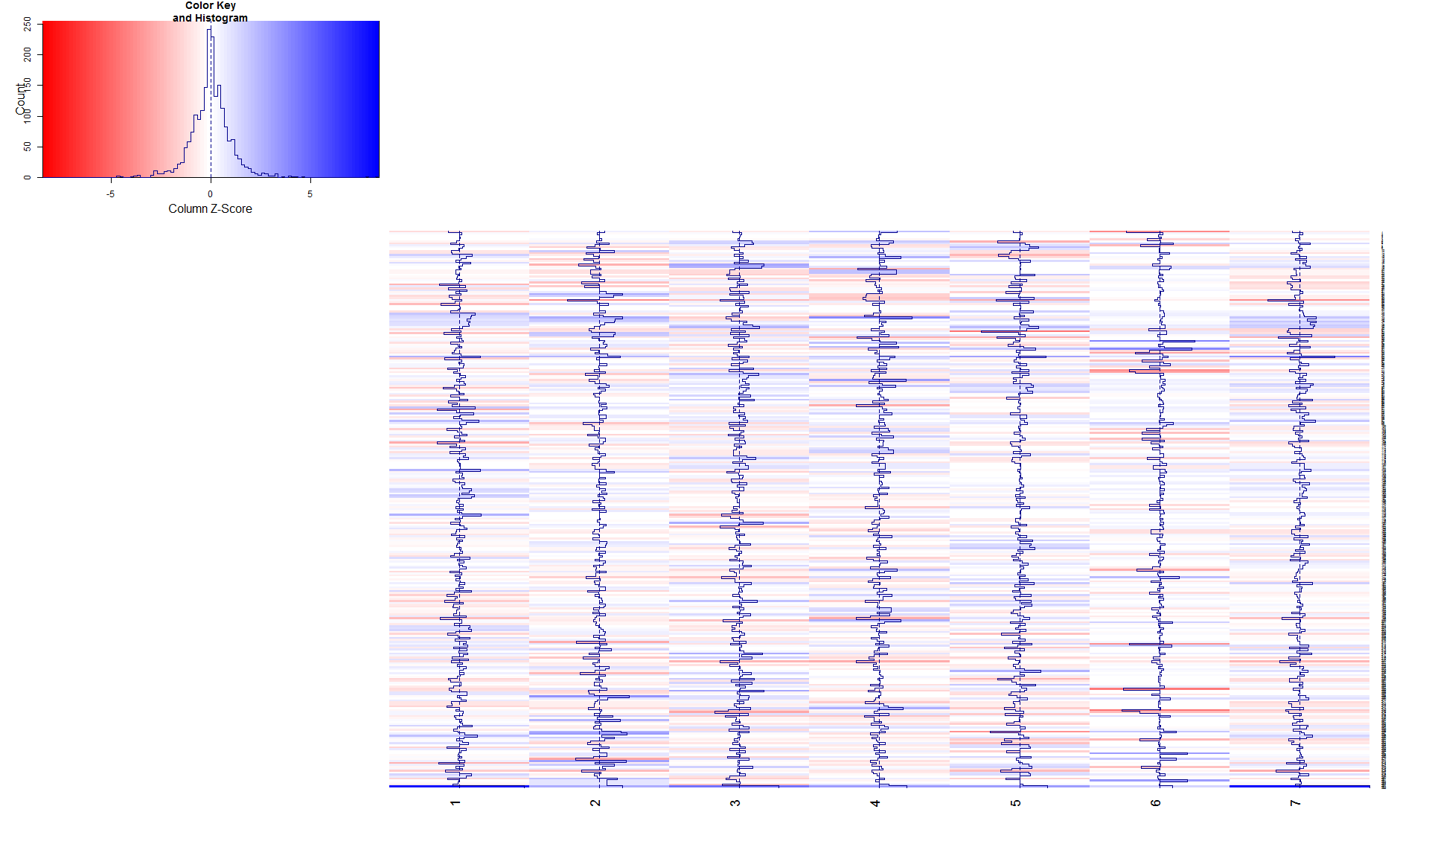
\includegraphics[width=1.1\columnwidth]{pattern}
%\end{figure}
%}
\subsection{Comparison with single-task model}
\frame{
\frametitle{Comparison with Ridge Regression}
\begin{figure}
  \centering
  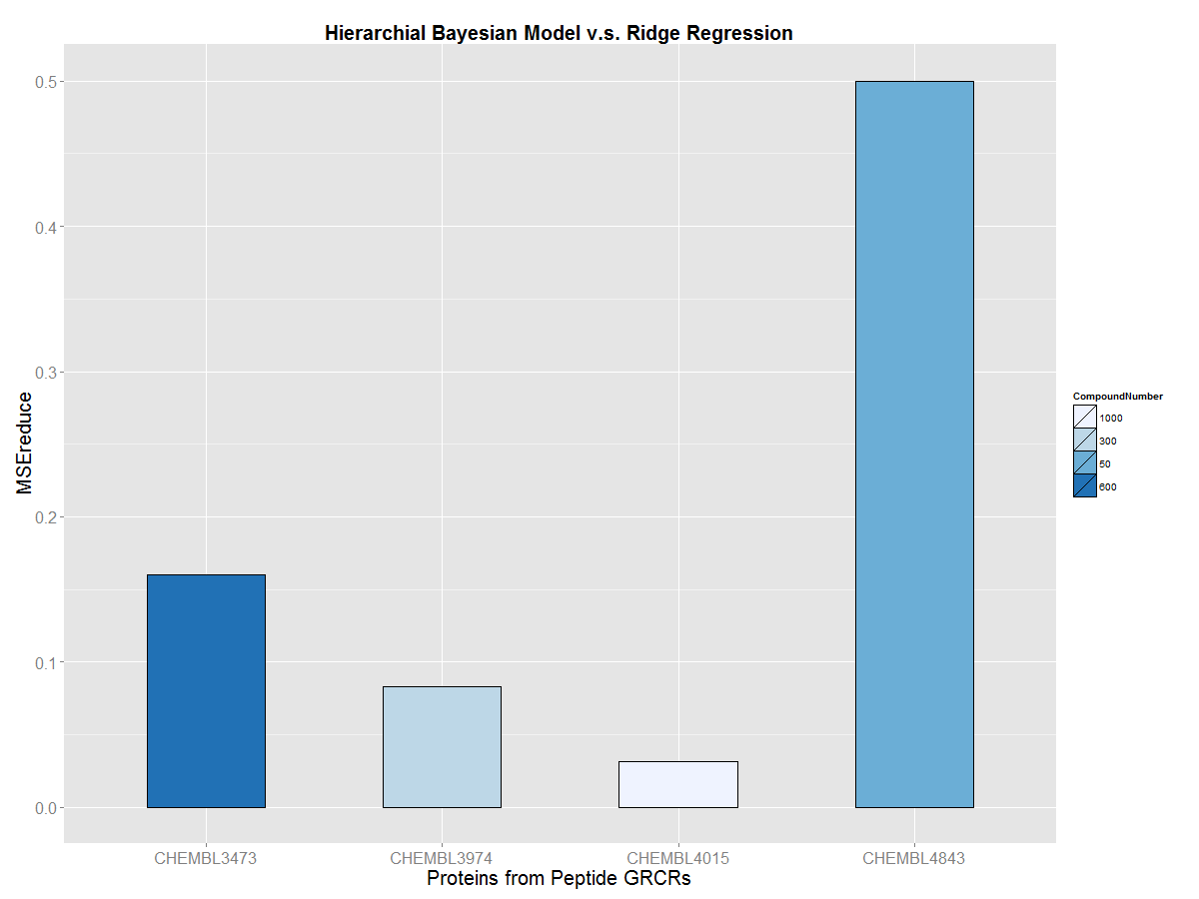
\includegraphics[width=0.9\columnwidth]{compare}
\end{figure}
}

\section{Discussion}
\frame{
\frametitle{Discussion}
\begin{itemize}
\item More compounds' fingerprints are being collected by the open-source chemoinformatics and machine learning package termed RDKit.
  %\item
  %A hierarchial Bayesian model is constructed to predict CPIs following the multi-task approach.
  %\item
  %More computational tests
  %\item
  %The relationship between proteins' pharmacological and genomic information
  \item
  Computational issue:
  \begin{itemize}
    \item
    High dimension v.s. Sparsity \\
    Colinearity
    \item
    Linear v.s. Nonlinear
  \end{itemize}
\end{itemize}
}
\end{document}